\documentclass{beamer}

\usetheme[hidefootline,altlogo=images/ssl-logo_text.png,nosidebar]{Oxford}
\usepackage{subcaption}

\begin{document}

\title[Exploiting Implicit Trust in Satellite Downlink Processing Systems]{Firefly: New Experimental Design}
\author[Edd Salkield]{
  \emph{Edd Salkield}
  \inst{1}
  \and
  Joshua Smailes
  \inst{1}
  \and
  Richard Baker
  \inst{1}
  \and
  Martin Strohmeier
  \inst{2}
  \and
  Ivan Martinovic
  \inst{1}
}
\institute[--~~Systems Security Lab]{
  \inst{1} Systems Security Lab, University of Oxford \and %
  \inst{2} Cyber-Defence Campus, armasuisse Science + Technology
}
\date{Michaelmas Term 2022}

\makeoxfordtitle

\section{Overview}

\begin{frame}
  \frametitle{Firefly 2.0}
  \framesubtitle{Research questions}

  \textit{Understanding the barriers to entry for signal injection attacks against the downlink}

  What are the main factors to consider regarding...
  \begin{itemize}
    \item an attacker getting their signal into the victim antenna?
    \item an attacker knowing that their signal will cause the intended harm?
    \item the downstream effects that an attacker can expect to cause?
  \end{itemize}
\end{frame}

\begin{frame}
  \frametitle{Firefly: overall paper structure}
  \framesubtitle{Experimental method}

  \begin{enumerate}
    \item Validate antenna attenuation model in the real world
    \item Understand how common protocols/decoders are weak to downlink injection
    \item End-to-end attack demonstration through amateur radio satellite
    \item Analyse downstream attack consequences
  \end{enumerate}
\end{frame}

% Ideally we would overshadow our own dish live, but for legal reasons that's slightly tricky

\section{Validate antenna attenuation model}

\begin{frame}
  \frametitle{Section 1: Validate antenna attenuation model}
  \framesubtitle{Summary}
  \textit{Validate antenna attenuation model and understand the key factors affecting injection capability}

  \centering
  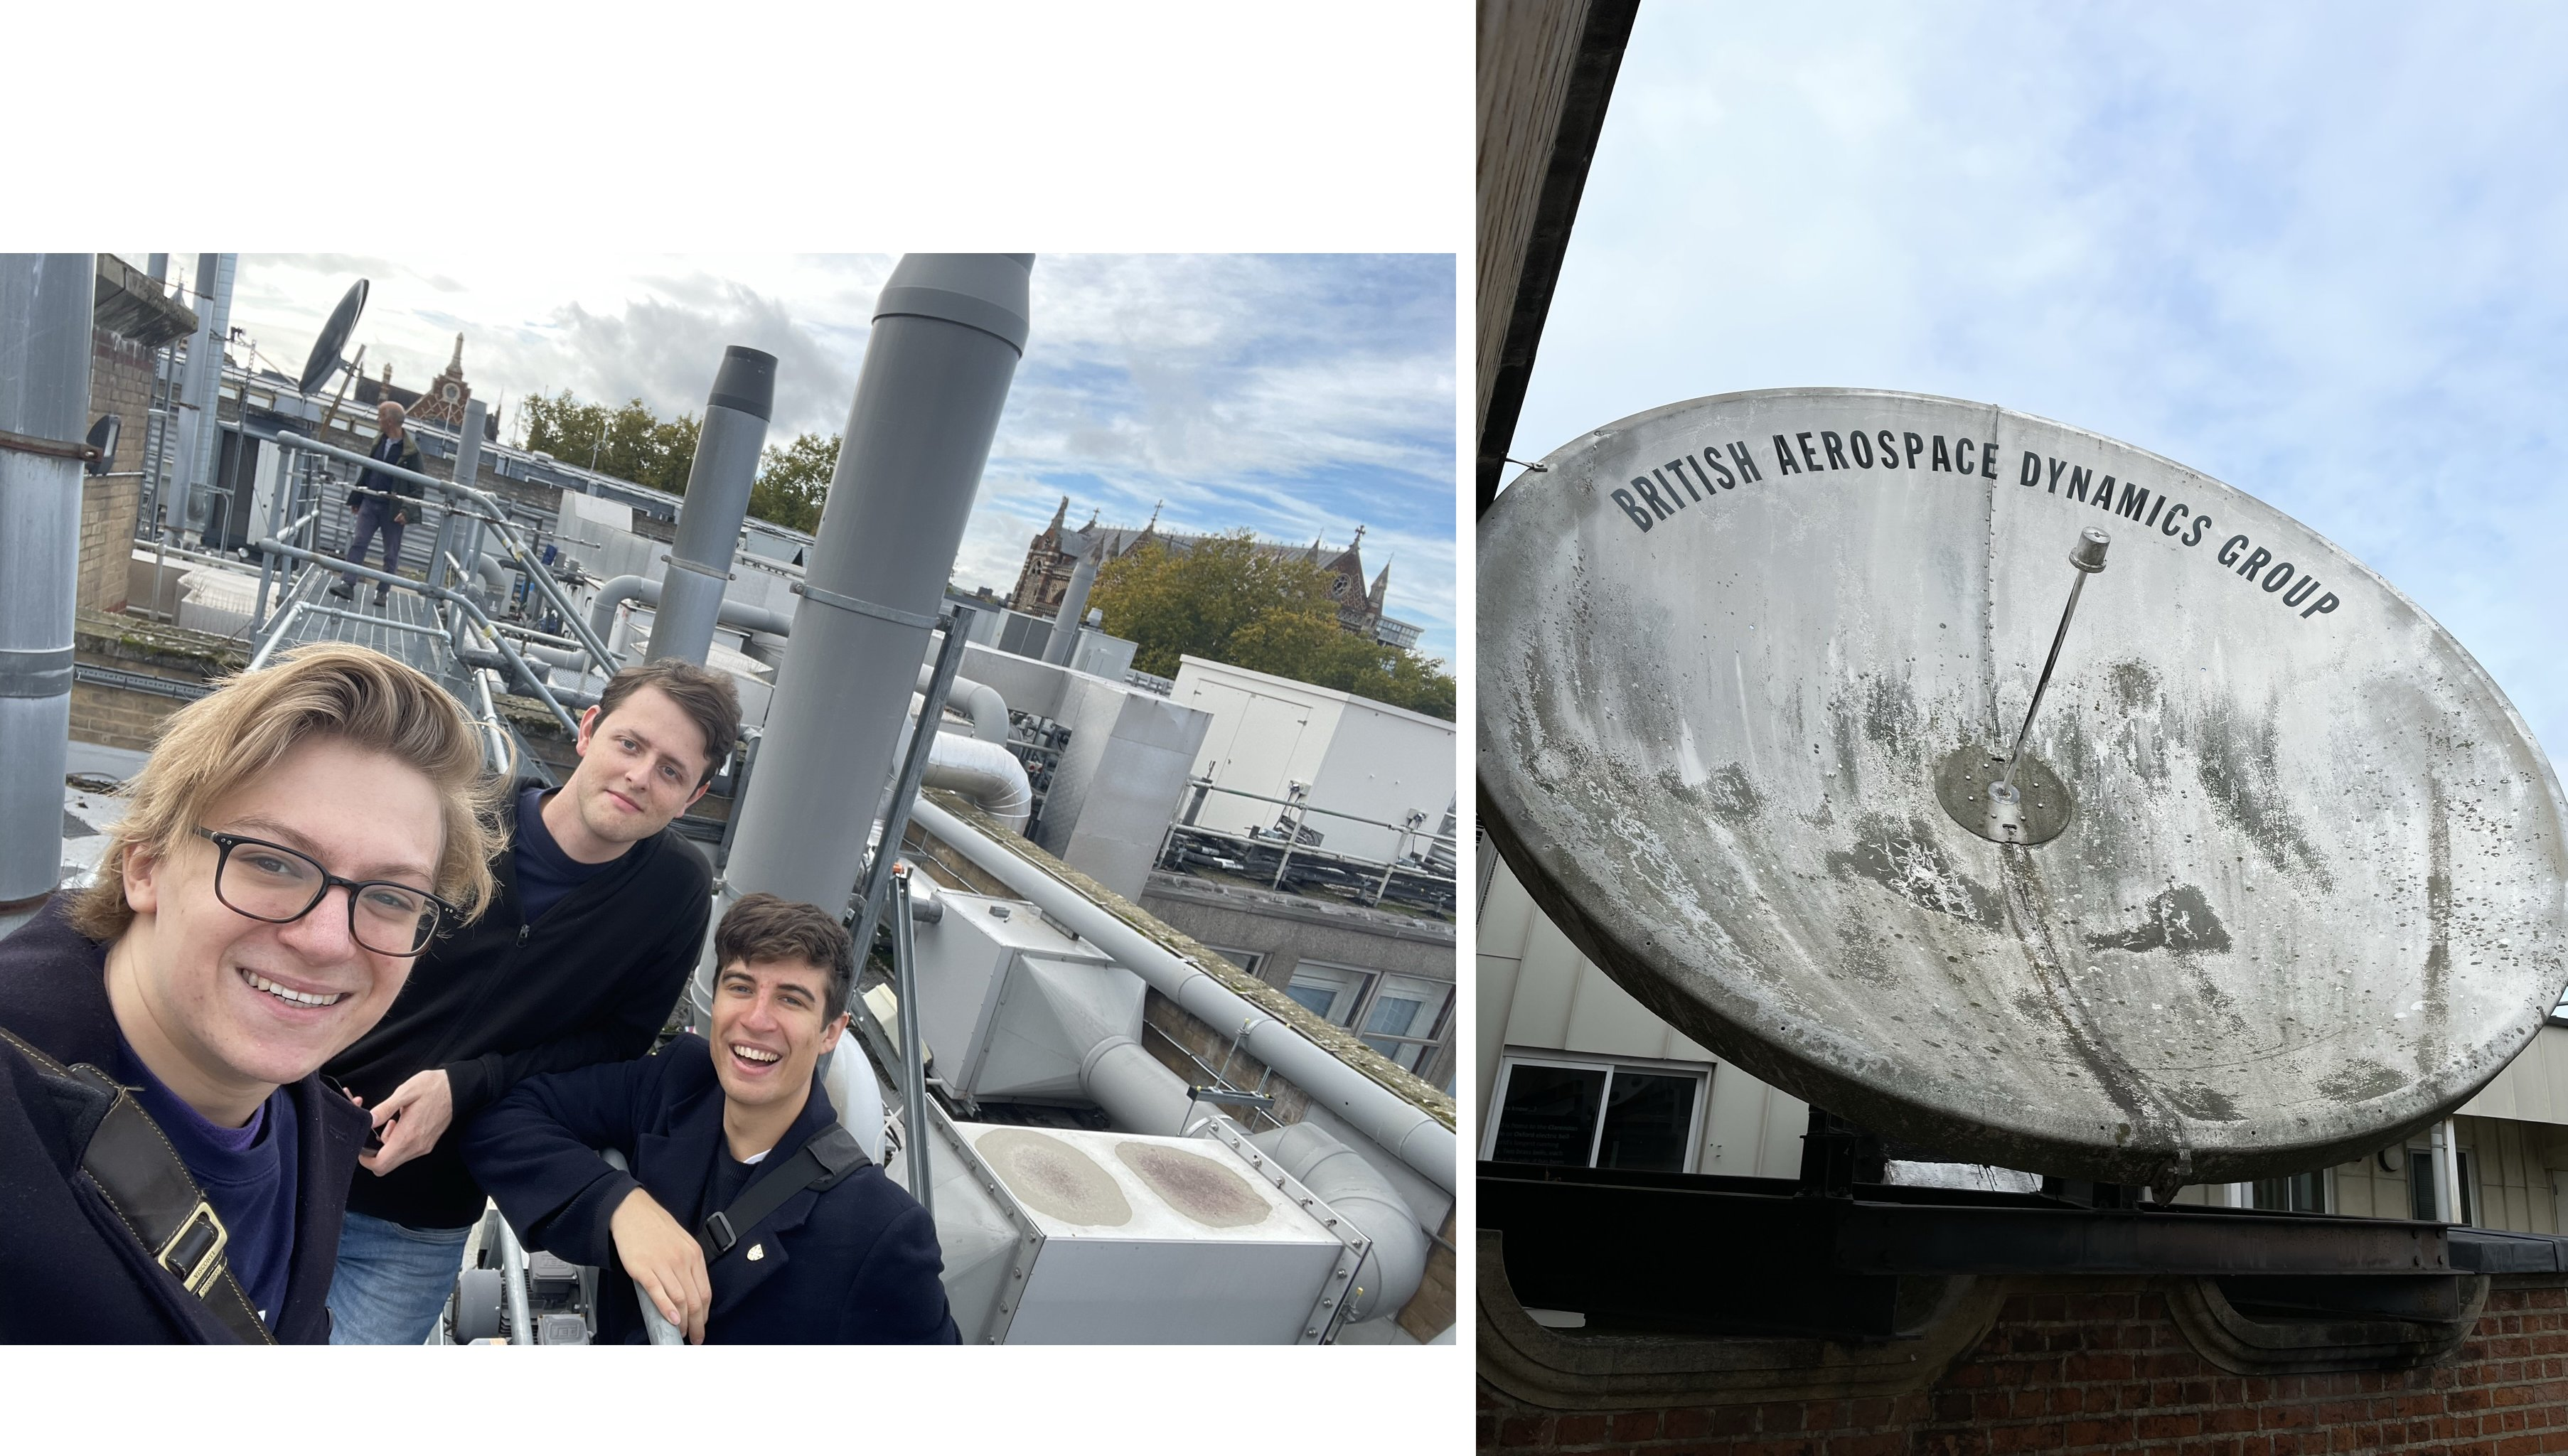
\includegraphics[width=0.8\columnwidth]{images/photos/dishes.jpg}

  Emit amateur-frequency signals at various antennas in real world settings and measure the gain/SNR
\end{frame}
\note{We currently have a model that the attacker can use, but we didn't validate it}

\begin{frame}
  \frametitle{Section 1: Physical layer}
  \framesubtitle{Experiment: Out-of-band angular emission}

  Method:
  \begin{itemize}
    \item Set up several antenna types in a real world setting
    \item Emit repeated, distinct legal out-of-band signals at the dish in amateur frequency bands
    \item Filter down to just the band that we emit, and measure signal gain before/after emission
  \end{itemize}
\end{frame}

\begin{frame}
  \frametitle{Section 1: Physical layer}
  \framesubtitle{Experiment: Out-of-band angular emission}

  Outcomes:
  \begin{itemize}
    \item A number of meaurements of gain/SNR in multiple injection settings
    \item Compare against the polar plots we get from simulation
    \item Understand how accurately the model lets an attacker estimate equipment needed beforehand
  \end{itemize}
\end{frame}

\section{Analyse weak protocols}

\begin{frame}
  \frametitle{Section 2: Analyse weak protocols}
  \framesubtitle{Summary}

  Outcome: Understand how common protocols/decoders are weak to injection on the downlink

  Summary: Reverse several protocols/decoders to determine packets that break things if injected

  Proposed work:
  \begin{itemize}
    \item Terra/Aqua (completed)
    \item Johannes' decoders
    \item Meteosat
    \item Iridium packets
  \end{itemize}
\end{frame}

\section{End-to-end attack demonstration}

\begin{frame}
  \frametitle{Section 3: End-to-end attack demonstration}
  \framesubtitle{Summary}

  Outcome: End-to-end attack to understand the key protocol factors affecting injection capability

  Summary: Overshadow reflected bent-pipe signal from QO-100 or equivalent at antenna gains calibrated to mirror the real-world setup, causing erroneous bytes to be decoded
\end{frame}

\begin{frame}
  \frametitle{Section 3: End-to-end attack demonstration}
  \framesubtitle{Experiment: overshadowing amateur satellite}

  Method:
  \begin{itemize}
    \item Create encoded physical-layer satellite signals
    \item Modulate the signals onto the uplink
    \item Overshadow the downlink with a calibrated signal
    \item Pipe the resulting decoding software into modems/decoding software
  \end{itemize}
\end{frame}

\begin{frame}
  \frametitle{Section 3: End-to-end attack demonstration}
  \framesubtitle{Transmitting}
  \centering
  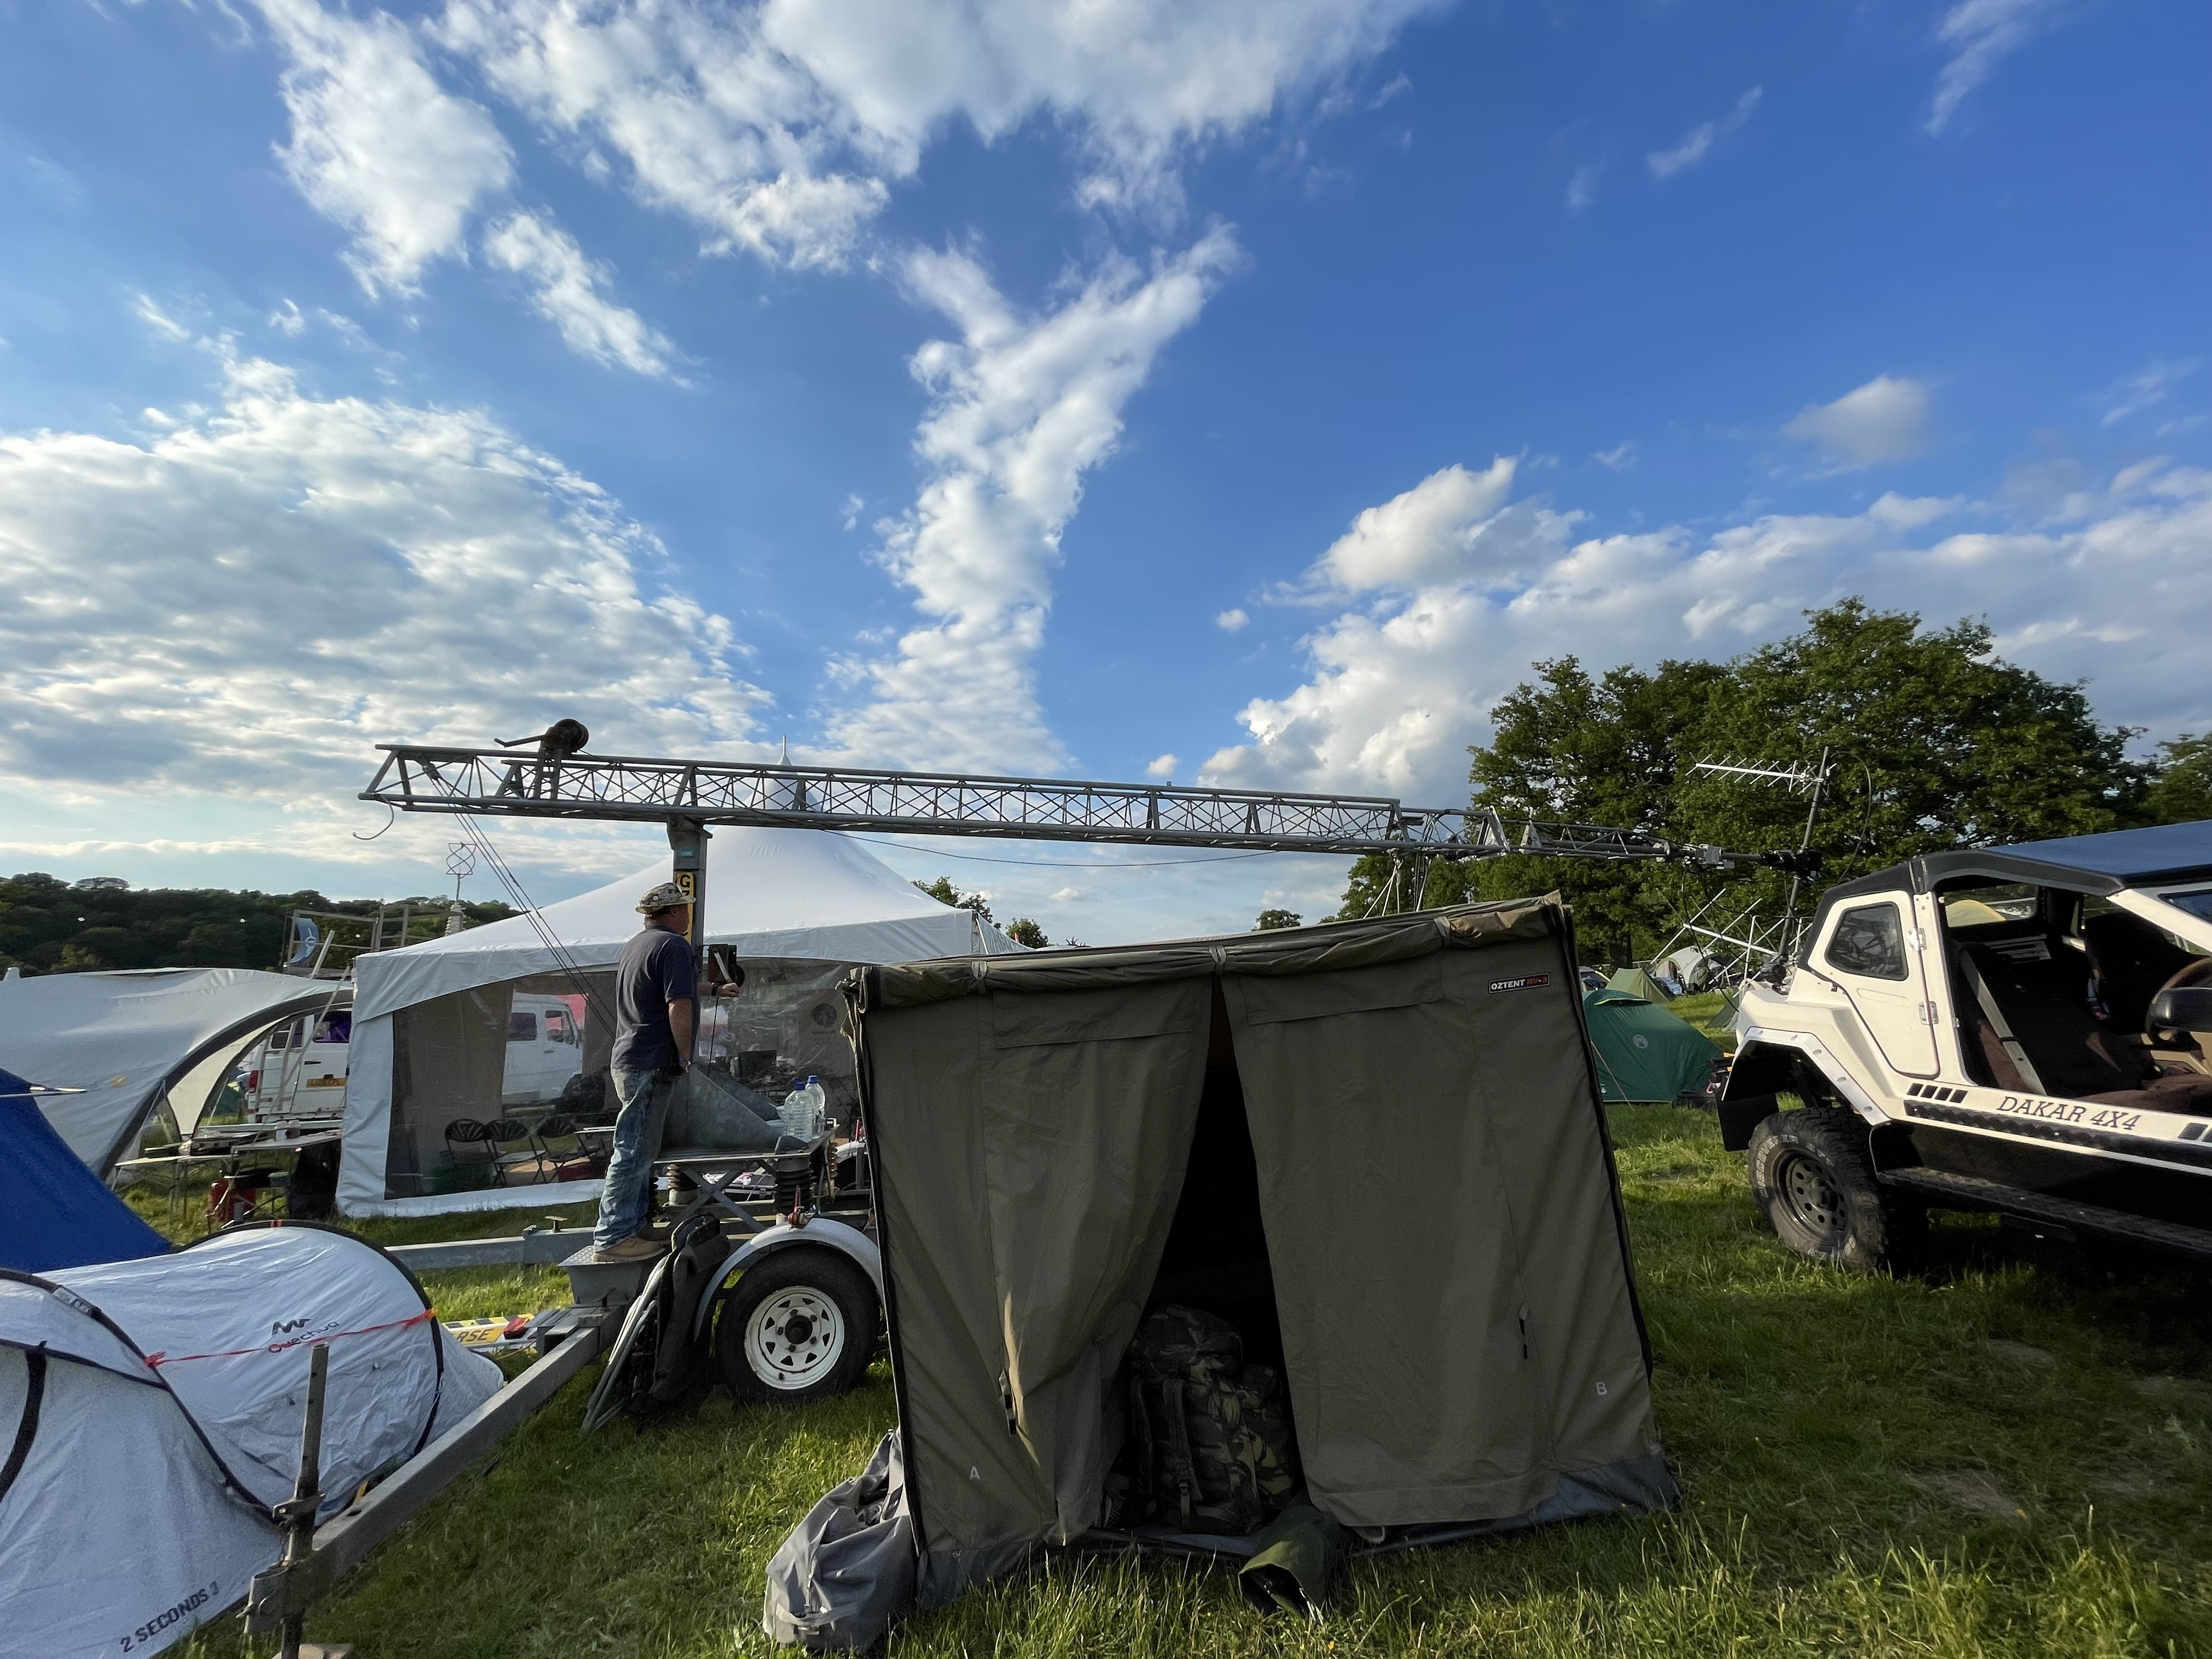
\includegraphics[width=0.6\columnwidth]{images/photos/emf_antenna.jpg}
\end{frame}

\begin{frame}
  \frametitle{Section 3: End-to-end attack demonstration}
  \framesubtitle{Overshadowing}
  Requirements:
  \begin{itemize}
    \item SDR (already in lab)
    \item X-band upconverter
    \item Amplifier
  \end{itemize}

  Options:
  \begin{itemize}
    \item COTS Dartcom X-Band system: ~90,000GBP\footnote{https://www.dartcom.co.uk/products/x-band-eos-system/technical-summary}
    \item Qorvo QPF5005EVB1: ~1600GBP
    \item Qorvo QPF5005: ~200GBP
  \end{itemize}
\end{frame}

\begin{frame}
  \frametitle{Section 3: End-to-end attack demonstration}
  \framesubtitle{Overshadowing}

  \centering
  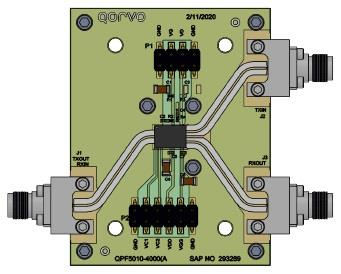
\includegraphics[width=0.6\columnwidth]{images/QPF5005EVB_SPL.jpg}
\end{frame}

\begin{frame}
  \frametitle{Section 3: End-to-end attack demonstration}
  \framesubtitle{Receiving}
  \centering
  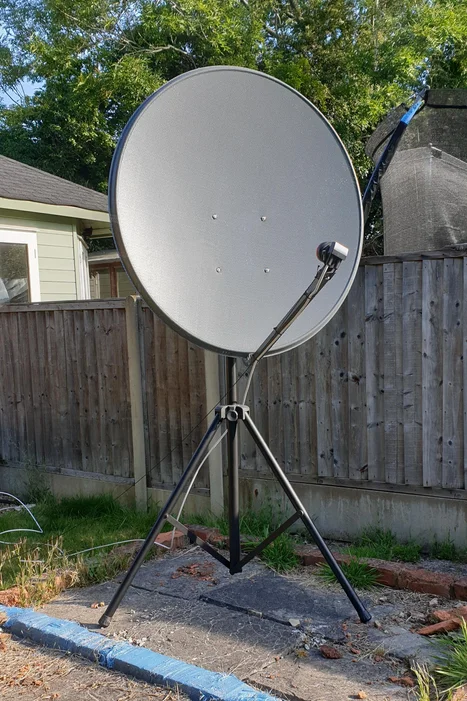
\includegraphics[width=0.5\columnwidth]{images/dish.png}
\end{frame}
\end{document}
